\section{Matrix-free multigrid}
  \label{section:applications:matrix-free-multigrid}

\chapterDescription
  {
    1--2 days.
  }
  {
    Chapter \ref{chapter:quickstart}. It is advantageous if the reader has
    studied the implementation of the heat equation before.
  }

In this section, we sketch how to solve the convection-diffusion equation
\[
  - \nabla (\epsilon \nabla) u + \nabla (v\ u) = f \qquad \mbox{with } v \in
  \mathbb{R}^d, \epsilon \in \mathbb{R}^{d \times d}
\]
with various geometric multigrid solvers. $epsilon$ is a diagonal matrix with
entries $\epsilon _1, \epsilon _2$ or $\epsilon _1, \epsilon _2, \epsilon _3$,
respectively.
Our realisation is based upon a few design decisions:

\begin{enumerate}
  \item The solvers use the spacetree as computational grid.
  \item We use a finite element formalism with $d$-linear shape functions.
  \item The material parameters $\epsilon $ and $v$ are given per cell.
\end{enumerate}


\noindent
For the implementation, we use Peano's \texttt{matrixfree} toolbox. 
This is a tiny little collection of helper classes to work with stencils and
local assembly matrix. 
It is neither fast, i.e.~computationally mature, nor can it cope with real
stencil libraries, but it does the job.



\subsection{Setup}

We start with Peano's PDT and generate a project. We also link Peano's sources
into the project and unzip the \texttt{matrixfree} toolbox. 
\begin{code}
  java -jar pdt.jar --create-project multigrid multigrid
  ln -s mypath/src/peano 
  ln -s mypath/src/tarch
  cp mypath/tarballs/toolboxes/matrixfree.tar.gz .
  tar -xzvf matrixfree.tar.gz
\end{code}


\noindent
I recommend to hold \texttt{matrixfree} parallel to the \texttt{multigrid},
\texttt{peano} and \texttt{tarch} directory.
As soon as we use such a toolbox, we also might have to adopt our makefile
accordingly: we have to add the matrixfree directory to the find pathes when we
build up a list of source codes.
Furthermore, you might have to add an additional search directory. If you place
your toolbox parallel to \texttt{peano} and \texttt{tarch}, this however should
not be necessary.
Here's the corresponding excerp from the makefile:
\begin{code}
files.mk:
    touch files.mk
    echo -n SOURCES= > files.mk
    find -H $(PEANO_HOME)/peano -name '*.cpp' | awk '{ printf "%s ", $$0 }' >> files.mk
    find -H $(PEANO_HOME)/tarch -name '*.cpp' | awk '{ printf "%s ", $$0 }' >> files.mk
    find -H $(PEANO_HOME)/matrixfree -name '*.cpp' | awk '{ printf "%s ", $$0 }' >> files.mk
    find $(PROJECT_HOME) -name '*.cpp' | awk '{ printf "%s ", $$0 }' >> files.mk
\end{code}

\noindent
We next add our material parameters to the \texttt{Cell.def} file
\begin{code}
Packed-Type: short int;

Constant: DIMENSIONS;

class multigrid::records::Cell {  
  persistent parallelise double   epsilon[DIMENSIONS];
  persistent parallelise double   v[DIMENSIONS];
};
\end{code}

\noindent
and create a simple first specification file:
\begin{code}
component: Multigrid

namespace: ::multigrid

vertex:
  dastgen-file: Vertex.def
  
cell:
  dastgen-file: Cell.def

state:
  dastgen-file: State.def

event-mapping:
  name: CreateGrid

event-mapping:
  name: PlotCells

adapter:
  name: CreateGrid
  merge-with-user-defined-mapping: CreateGrid
  merge-with-user-defined-mapping: PlotCells
  
\end{code}

\noindent
We run this specification file through the PDT

\begin{code}
java -jar <mypath>/pdt.jar --generate-gluecode multigrid/project.peano-specification multigrid
\end{code}


\noindent
and implement both the plotter and the creational mapping such that we have a
few characteristic setups. 
It might however make sense to validate that make passes before we start any
PDE-specific coding:
\begin{code}
make -f multigrid/makefile
\end{code}


\noindent
We next introduce an operation 
\begin{code}
matrixfree::stencil::ElementWiseAssemblyMatrix multigrid::Cell::getElementsAssemblyMatrix(
  const tarch::la::Vector<DIMENSIONS,double>&  h
) const {
  matrixfree::stencil::ElementWiseAssemblyMatrix result;

  const matrixfree::stencil::Stencil laplacianStencil = 
    matrixfree::stencil::getLaplacian(_cellData.getEpsilon(), h);

  return matrixfree::stencil::getElementWiseAssemblyMatrix(laplacianStencil);
}
\end{code}
which returns the $\mathbf{R}^{2^d \times 2^d}$ local system matrix. 
The method sets up the stencils that correspond to a regular Cartesian system
given the mesh size \textt{h} and the material parameters.
Here, also the convective term has to be handled.
Finally, it uses \texttt{getElementWiseAssemblyMatrix} to extract the actual
matrix from this stencil.

\begin{remark}
  Peano supports all stencil/linear algebra operations for complex values.
\end{remark}


\subsection{Jacobi smoother}

The basic building block of all of our solvers is a simple Jacobi smoother
working on adaptive grids as well as on multiple scales.
Its realisation is an extension of the solver in \ref{section:applications:heat-equation}.
To make it work without the assembly of any global matrix, we associate each
vertex a residual value as well as the actual value. 
There are a few other features such as boundary properties or some level
analysis that we either use later on or we pass to the used toolboxes. 
Their exact semantics and rationale have to be taken from the source code.

\begin{code}
Packed-Type: short int;


class multigrid::records::Vertex {  
  /**
   * Solution
   */
  persistent parallelise double  u;

  /**
   * Rhs
   */
  persistent parallelise double  f;
  
  /**
   * Residual
   */
  persistent parallelise double   r;

  /**
   * Diagonal element
   */
  persistent parallelise double   d;
  
  enum VertexType {
    Unknown, Dirichlet, Neumann
  };
  
  persistent VertexType vertexType;
  
  // some other attributes
};
\end{code}

\noindent
Besides a proper initialisation of the vertices, we extend the specification
similar to the heat equation.
\begin{code}
component: Multigrid

namespace: ::multigrid

vertex:
  dastgen-file: Vertex.def
  read scalar(double): U
  read scalar(double): R
  read scalar(double): D
  read scalar(double): F
  write scalar(double): U
  write scalar(double): R
  write scalar(double): D
  
...

adapter:
  name: CreateGrid
  merge-with-user-defined-mapping: CreateGrid
  merge-with-user-defined-mapping: PlotCells
  merge-with-predefined-mapping: VTKPlotVertexValue(u,getU,u)
\end{code}

\noindent
Once this code framework passes (only minor technical helper routines have to
be implemented, but by now this should be straightforward to any user), we can
introduce a new mapping/adapter \texttt{JacobiSmoother}, call this one a couple of hundred times in the runner and plot the result file then. 
For the latter, it makes sense to use a predefined plotter.
The interesting new aspects can be found in three routines of the smoother.
The design of the code realises matrix-free element-wise mat-vecs 1:1: 


\begin{enumerate}
  \item Each vertex carries a residual and a diagonal value attribute. 
    They are cleared whenever the vertex is read the very first time in
    a traversal.
    \begin{code}
void multigrid::mappings::JacobiSmoother::touchVertexFirstTime(...) {
  logTraceInWith6Arguments( "touchVertexFirstTime(...)", ... );

  fineGridVertex.clearAccumulatedAttributes();

  logTraceOutWith1Argument( "touchVertexFirstTime(...)", fineGridVertex );
}

// in Vertex files

void multigrid::Vertex::clearAccumulatedAttributes() {
  _vertexData.setR(0.0);
  _vertexData.setD(0.0);
}
    \end{code}
    
    \noindent
    Our concept is that we accumulate the diagonal element $d$ and the residual
    $r$ within these (temporary) attributes per vertex throughout the traversal.
    
    \item When we use a vertex for the very last time, we may thus update the
    unknown according to the values of the residual and the diagonal value. This
    is the actual Jacobi smoothing step:
    \[
      u ^{(new)} \gets u ^{(old)} + \omega \frac{1}{d} r
    \]
    \begin{code}
void multigrid::mappings::JacobiSmoother::touchVertexLastTime(...) {
  const bool hasUpdated = fineGridVertex.performJacobiSmoothingStep( omega );
  
  ...
}

// in Vertex files

double multigrid::Vertex::getResidual() const {
  return _vertexData.getF() + _vertexData.getR();
}


bool multigrid::Vertex::performJacobiSmoothingStep( double omega ) {
  if (
    getRefinementControl()==Vertex::Records::Unrefined
    &&
    _vertexData.getVertexType()== Records::Unknown
  ) {
    assertion1( _vertexData.getD()>0.0, toString() );
    assertion2( omega>0.0, toString(), omega );
    _vertexData.setU( _vertexData.getU() + omega / _vertexData.getD() * getResidual() );
    return true;
  }
  else {
    return false;
  }
}
    \end{code} 
    
    \noindent
    Please note that the residual here is modelled as sum of the right-hand
    side and the accumulated value (cf.~helper operation
    \texttt{getResidual()}).
    We anticipate the minus from the definition 
    \[ r = f - Au \]
    already in the accumulation, i.e.~sum up $-Au$ in the vertex attribute $r$.
    An additional pitfal is this context stems from the usage of a finite
    element method.
    It implies that we have to ensure that $f$ is scaled with $h^d$ ($h$ being the local mesh width), which is something we typically
    do already in the initialisation. 
    
    \begin{remark}
    It is obvious that the Jacobi update scheme may only update inner
    unrefined vertices as well as Neumann boundary points. Peano does not offer
    vertex types. It distinguishes only inner and outer vertices. As we need
    more flags than inside and outside (at least two boundary
    flags), we have to offer these on our own\footnotemark .
    \end{remark}
    \footnotetext{Up to
    early 2016, Peano had a three-valued logic with inner, outer and boundary vertices. I
    removed this from the kernel as most applications need way more vertex
    types anyway.}
    
    
    In the present implementation, we make the Jacobi update return a flag that
    indicates whether a fine grid update has been done or not. 
    Most codes will like to track global data such as a global residual or the
    maximum value of the solution and can use this flag to decide whether a
    vertex contributes to global data or not. Please study the accompanying
    source code for details.
    
    \item The most complicated part is obviously the evaluation of the local
    mat-vec contributions. Here, we rely on the cell's
    \texttt{getElementsAssemblyMatrix} as well as operations from \newline
    \texttt{VertexOperations}. All operations in this class are generated by the
    PDT and extract from \texttt{enterCell}'s vertices vectors: you hand in all
    fine grid data and extract a vector of all $u$ values, e.g. The other way
    round is supported as well. The operations within this helper class are all
    generated because of the read and write statements in the specification. 
    \begin{code}
#include "multigrid/VertexOperations.h"

void multigrid::mappings::JacobiSmoother::enterCell(...) {
  logTraceInWith4Arguments( "enterCell(...)", fineGridCell, ... );

  const tarch::la::Vector<TWO_POWER_D,double> u    =
    VertexOperations::readU( fineGridVerticesEnumerator, fineGridVertices );
  const tarch::la::Vector<TWO_POWER_D,double> dOld    =
    VertexOperations::readD( fineGridVerticesEnumerator, fineGridVertices );
  const tarch::la::Vector<TWO_POWER_D,double> rOld =
    VertexOperations::readR( fineGridVerticesEnumerator, fineGridVertices );
  const matrixfree::stencil::ElementWiseAssemblyMatrix A =
    fineGridCell.getElementsAssemblyMatrix( fineGridVerticesEnumerator.getCellSize() );

  tarch::la::Vector<TWO_POWER_D,double> r = rOld - A * u;
  tarch::la::Vector<TWO_POWER_D,double> d = dOld + tarch::la::diag(A);

  VertexOperations::writeR( fineGridVerticesEnumerator, fineGridVertices, r );
  VertexOperations::writeD( fineGridVerticesEnumerator, fineGridVertices, d );

  logTraceOutWith1Argument( "enterCell(...)", fineGridCell );
}
    \end{code}
\end{enumerate}



\subsection{Environment}

The changes in the environment are straightforward once the smoother is 
in place:
\begin{enumerate}
  \item We extend the runner such that it switches to the Jacobi smoother once 
  the grid is set up and triggers a fixed number of iterations then.
  \item We add a logging device to the runner
  \begin{code}
    class multigrid::runners::Runner {
      private:
        static tarch::logging::Log  _log;
        ...
    };
  \end{code}
  and make the innermost loop plot residual and other statistics after each 
  grid traversal:
  \begin{code}
  repository.switchToJacobiAndPlot();
  for (int i=0; i<100; i++) {
    repository.iterate();

    logInfo(
      "runAsMaster(...)",
      "#vertices=" << repository.getState().getNumberOfInnerLeafVertices() <<
      ",|res|_2=" << repository.getState().getResidualIn2Norm() <<
      ",|res|_max=" << repository.getState().getResidualInMaxNorm() <<
      ",|u|_L2=" << repository.getState().getSolutionInL2Norm() <<
      ",|u|_max=" << repository.getState().getSolutionInMaxNorm() <<
      ",#stencil-updates=" << repository.getState().getNumberOfStencilUpdates()
    );

    repository.getState().clearAccumulatedAttributes();
  }
  \end{code}
  \item To make the code work, we augment the state with the corresponding
  fields 
  \begin{code}
Packed-Type: short int;

class multigrid::records::State {  
  // Stores squared value, i.e. apply sqrt before returning it
  persistent parallelise double residual2Norm;
  persistent parallelise double residualMaxNorm;
  // Stores squared value, i.e. apply sqrt before returning it
  persistent parallelise double solutionL2Norm;
  persistent parallelise double solutionMaxNorm;
  persistent parallelise double numberOfStencilUpdates;
};
  \end{code}
  and realise the corresponding setters and getters. The design of the state
  methods (notably a method \texttt{clearAccumulatedAttributes()} in
  combination with \texttt{merge}) follows recommendations motivated in Section
  \ref{section:parallelisation:shared-memory}. For the time being, we do not
  discuss them further.
  \item Finally, we extend the \texttt{main} such that it can read in a
  well-suited relaxation parameter from the command line. It then sets this
  relaxation parameter (the static field) in the mapping:
  \begin{code}
    multigrid::mappings::JacobiSmoother::omega = atof( argv[2] );
  \end{code}
\end{enumerate}


\noindent
We may run this code for example the
well-known Poisson benchmark ($\epsilon = 1, v=0, f=d\ \pi ^2 \prod _i \sin
\left( x_i \pi \right) $ ), and observe the well-known dependency of Jacobi on
the mesh width (below grids with two, three or four compute grid levels):

\begin{center}
  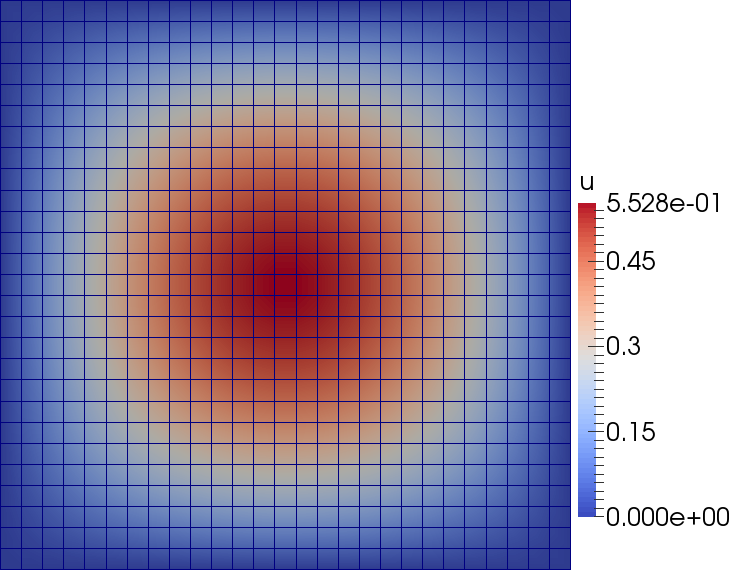
\includegraphics[width=0.3\textwidth]{42_matrix-free-multigrid/Poisson3.png}
  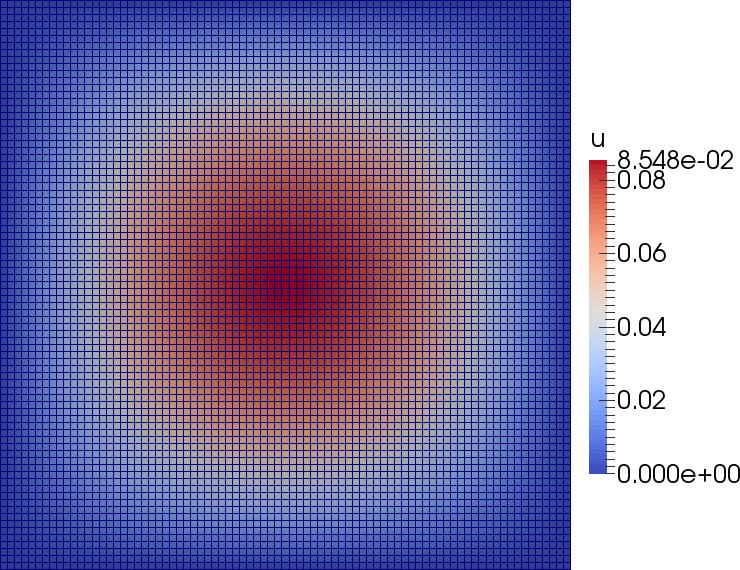
\includegraphics[width=0.3\textwidth]{42_matrix-free-multigrid/Poisson4.png}
  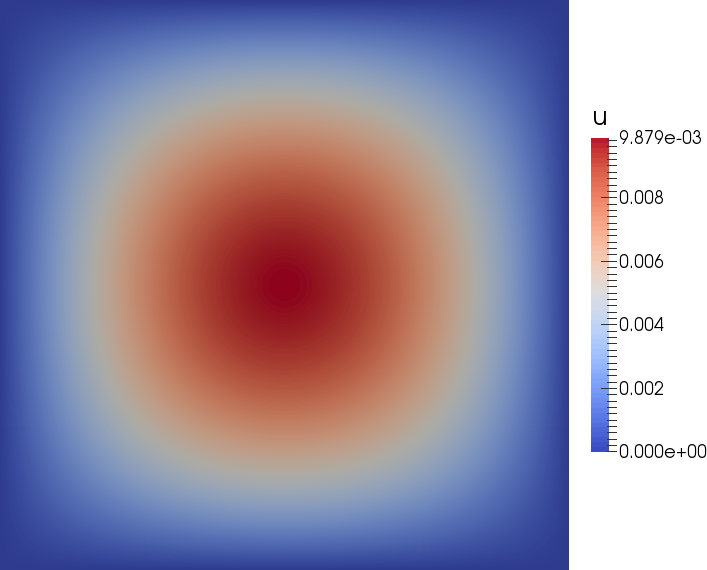
\includegraphics[width=0.3\textwidth]{42_matrix-free-multigrid/Poisson5.png}
\end{center}


\subsection{Dynamically adaptive Jacobi mit FAC}

\noindent 
We next implement a dynamically adaptive Jacobi solver that implements the FAC
scheme.
Its fundamental idea is that the Jacobi smootherr is applied on each and every
grid level in parallel.
Any hanging node's value is interpolated from coarser grids.
While we update all grid levels, we do overwrite coarse vertices with fine grid
values for all vertices that do exist on finer grid resolutions as well.
We inject the solution from the fine grids onto coarser grids.
This first solver is capable to handle dynamically adaptive grids with
arbitrary refinement pattern.
It also is a preliminary exercise how to implement multigrid full approximation
storage (FAS).

We extend the grid setup slightly such that it creates a very coarse grid even
if we prescribe a fine minimum mesh size.
Next, we validate that \texttt{enterCell} evaluates the stencil on each grid
level anyway.
This leaves two tasks incomplete: interpolatation and injection.
The injection is basically the same we have used in the heat equation before:
\begin{code}
void multigrid::mappings::JacobiSmoother::touchVertexLastTime(...) {
 // see code snippets introduced before

 if (
  peano::grid::SingleLevelEnumerator::isVertexPositionAlsoACoarseVertexPosition(
    fineGridPositionOfVertex
  )
 ) {
  const peano::grid::SingleLevelEnumerator::LocalVertexIntegerIndex coarseGridPosition =
    peano::grid::SingleLevelEnumerator::getVertexPositionOnCoarserLevel
    (fineGridPositionOfVertex);
  coarseGridVertices[ coarseGridVerticesEnumerator(coarseGridPosition) ].inject(fineGridVertex);
 }
}


// in the vertex

void multigrid::Vertex::inject(const Vertex& fineGridVertex) {
  _vertexData.setU( fineGridVertex._vertexData.getU() );
}
\end{code}



\begin{remark}
  The \texttt{matrixfree} toolbox offers a type \texttt{solver::Smoother} that
  realises a Jacobi smoother that automatically tracks different residual and
  solution norms. In the present example we do not use this smoother while we
  use the toolbox's multigrid class. This is kind of inconsistent. It would
  probably be better to use the smoother as well.
\end{remark}

\noindent
The interpolation follows the idea of the heat equation solver, too.
However, we propose to rely on a premanufactored interpolation operation from
the \texttt{matrixfree} toolbox.
For this, we make our smoother mapping hold an instance of
\texttt{matrixfree::solver::Multigrid  \_multigrid}.
This object in tun 

\begin{code}
void multigrid::mappings::JacobiSmoother::createHangingVertex(...) {
  logTraceInWith6Arguments( "createHangingVertex(...)", ... );

  fineGridVertex.setU(
    _multigrid.getDLinearInterpolatedValue(
      VertexOperations::readU( coarseGridVerticesEnumerator, coarseGridVertices ),
      fineGridPositionOfVertex
    )
  );

  logTraceOutWith1Argument( "createHangingVertex(...)", fineGridVertex );
}
\end{code}


\noindent
Obviously, the vertex requires an additional \texttt{setU( double )} operation.
But that's the only additional extension required.
If we adopt the setup, we should obtain start grids alike:

\begin{center}
  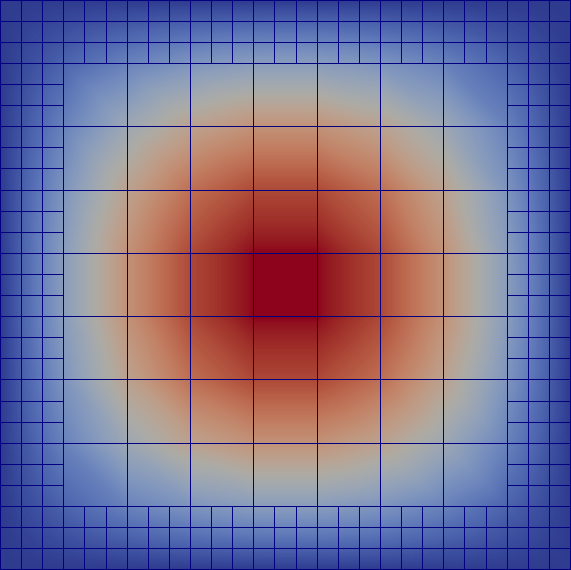
\includegraphics[width=0.3\textwidth]{42_matrix-free-multigrid/AdaptivePoisson3.png}
  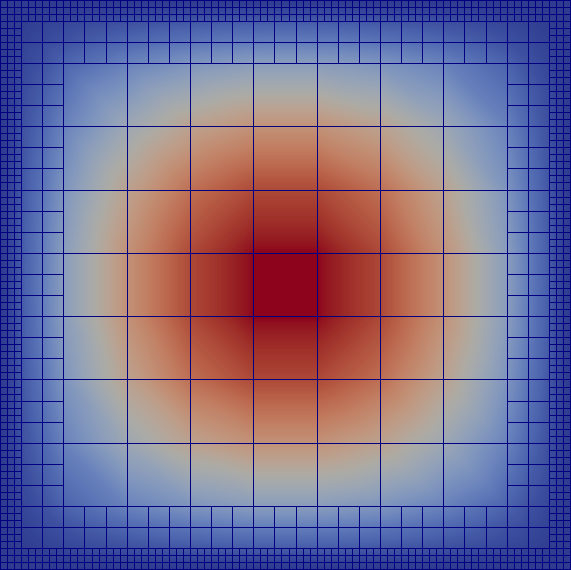
\includegraphics[width=0.3\textwidth]{42_matrix-free-multigrid/AdaptivePoisson4.png}
  \includegraphics[width=0.3\textwidth]{42_matrix-free-multigrid/AdaptivePoisson5.png}
\end{center}


\noindent
We close our discussion on the Jacobi smoother with the introducton of a dynamic
refinement criterion.
For this, we rely on a predefined refinement criterion offered with the
matrixfree toolbox.
We use
\texttt{matrixfree::adaptivitycriteria::LinearSurplusRefinementCriterionWithFixedMeshSizes}.
There is an extensive documentation how to use it in its superclass' header, so
we do not reiterate this here.

One final remark is worth trying: We have so far always used a
predefined visualisation routine that visualises the finest grid of a
simulation.
Among the set of standard visualisation routines also is a plotter that plots
the individual levels of a grid.
Given that we inject the solution to coarse levels anyway, this allows us to
visualise all data in a multilevel fashion.
To use it, we again extend our specification, regenerate the glue code and
recompile.

\begin{code}
adapter:
  name: JacobiAndPlot
  merge-with-user-defined-mapping: CreateGrid
  merge-with-user-defined-mapping: JacobiSmoother
  merge-with-user-defined-mapping: PlotCells
  merge-with-predefined-mapping: VTKPlotVertexValue(u,getU,u)
  merge-with-predefined-mapping: VTKPlotVertexMultilevelValue(multiscaleU,getU,u)
\end{code}




Adaptives Verfeineren. Dann muss man richtig interpolieren bei neuen Werten,
sonst gibt es Kaese





\subsection*{Further reading}

\begin{itemize}
  \item  Reps, Bram and Weinzierl, Tobias: {\em Complex additive geometric
  multilevel solvers for Helmholtz equations on spacetrees}, tech report,  
  arXiv:1508.03954
  \item Weinzierl, Marion: {\em Hybrid Geometric-Algebraic Matrix-Free Multigrid on
Spacetrees}, Dissertation, Technische Universit\"at M\"unchen, 2013
  \item   Muntean, Ioan Lucian, Mehl, Miriam, Neckel, Tobias and Weinzierl,
  Tobias (2008). {\em Concepts for Efficient Flow Solvers Based on Adaptive
  Cartesian Grids}. In High Performance Computing in Science and Engineering, Garching 2007. Wagner, Siegfried, Steinmetz, Matthias, Bode, Arndt & Brehm, Matthias Berlin Heidelberg New York: Springer.
  \item Weinzierl, Tobias and K\"oppl, Tobias (2012). {\em A Geometric
  Space-time Multigrid Algorithm for the Heat Equation}. Numerical Mathematics:
  Theory, Methods and Applications 5(1): 110-130.
  \item Mehl, Miriam, Weinzierl, Tobias and Zenger, Christoph (2006). {\em A
  cache-oblivious self-adaptive full multigrid method}. Numerical Linear Algebra
  with Applications 13(2-3): 275-291.
\end{itemize}
